\section{Metadades}\label{sec:metadata}

Les metadades són el conjunt d'etiquetes presents a qualsevol registre que contenen informació sobre aquest.
Els autors, la descripció del recurs, la data de pujada, el departament responsable, el tipus de document, o més, es troben inclosos. \\

\noindent
En el nostre cas, a \gls{UPCommons}, aquestes utilitzen el format \gls{DSpace} Intermediate Metadata, \gls{DIM}, que es basa en fer sservir el format Dublin Core incorporant un qualificador, amb la finalitat d'afinar la informació que inclous.
L'estructura és la següent:

\begin{figure}[htbp]
    \centerline{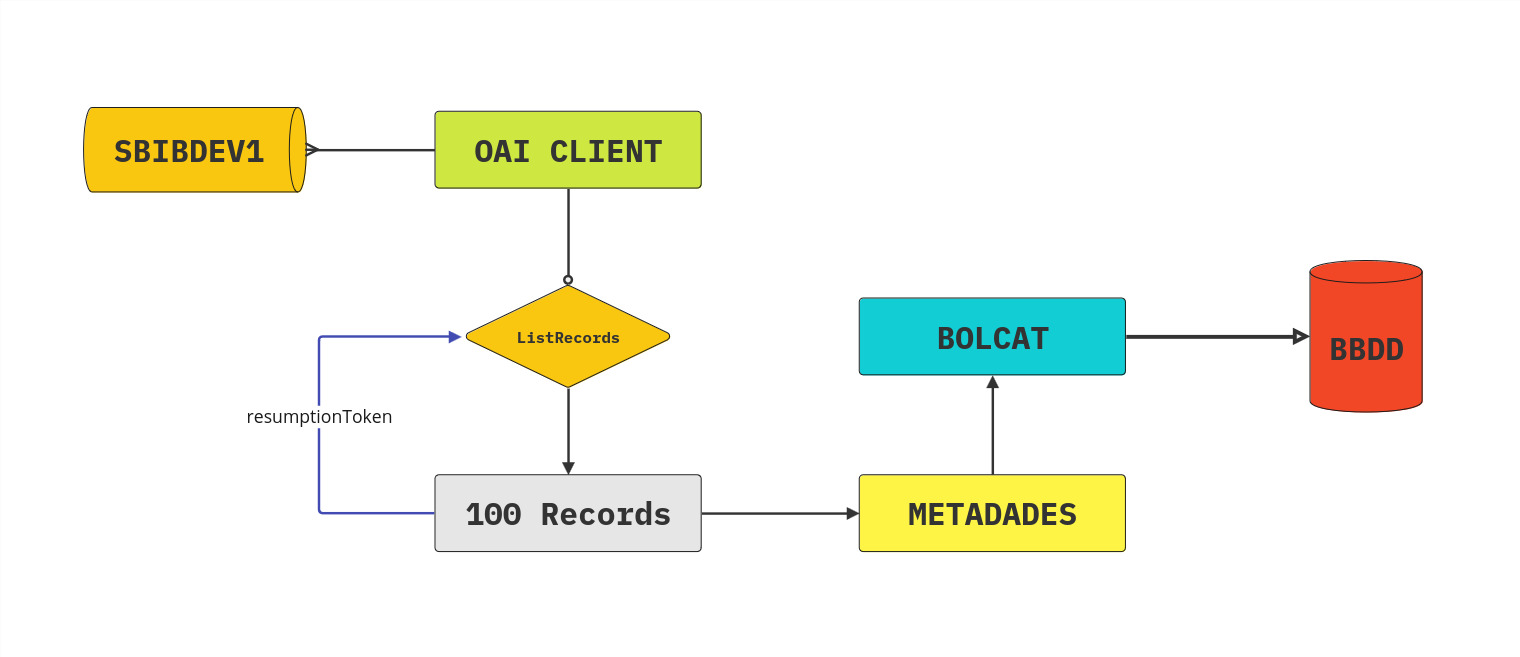
\includegraphics[width=1.2\textwidth]{figures/metadata-processing}}
    \captionsetup{justification=centering}
    \caption{Disseny tècnic del processament de les metadades.}\label{fig:log-analysis}
    \source{Elaboració pròpia.}
\end{figure}
